If we were to (hypothetically) measure a pressure drop of $6.35 mbar$ across the orfice plate with $C_d \approx 0.363 m^{-1}$ you would get a volume flow rate of $Q\approx 9.80\cdot 10^{-6} m^3/s$
\begin{figure}[h!]
    \centering
    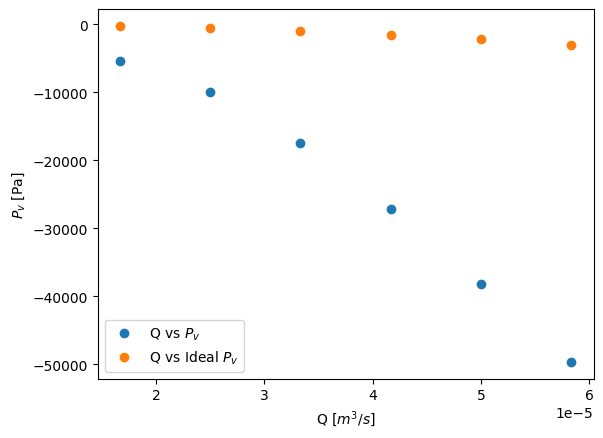
\includegraphics[width=60mm]{Diagrams/PvVsQ.png}
    \caption{Plot of measured $p_v$ vs $Q$ and and ideal $p_v$ vs $Q$}
    \label{fig:pvVsQ}
\end{figure}

\begin{table}[h!]
\resizebox{\columnwidth}{!}{%
\input{}
}
\caption{Table of calculated $h_{f1}$ and h_{f2}-values using equation \ref{eq:hf1} and \ref{eq:hf2}}
\label{table:hf1hf2}


\end{table}


\begin{figure}[h!]
    \centering
    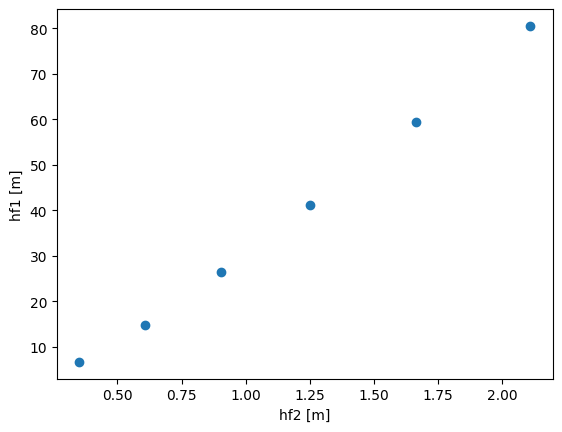
\includegraphics[width=60mm]{Diagrams/hf1Vshf2.png}
    \caption{Plot of $h_{f1}$ vs $h_{f2}$}
    \label{fig:hf1Vshf2}
\end{figure}


\begin{figure}[h!]
    \centering
    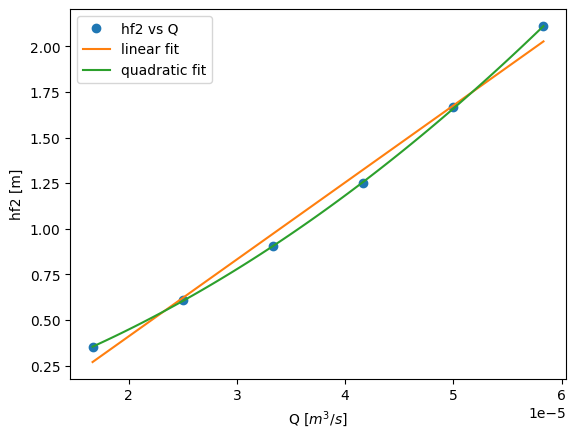
\includegraphics[width=60mm]{Diagrams/hf2VsQ.png}
    \caption{Plot of $h_{f2}$ vs $Q$ Including both linear $(a\cdot x+b)$ and quadratic fit$(a\cdot x^2 + b\cdot x^2 +c )$}
    \label{fig:hf2VsQ}
\end{figure}

